\subsection{トルクと粒子の回転}
\label{sec:rotation}
$xy$平面上を$x$軸方向に流れるせん断流下に球形粒子が存在する場合,
流体から受けるトルクは式\eqref{eq:hydro_torque_z}で表される\cite{hidro_torque}.
    \begin{equation}
        N^\mathrm{H}_z = 4 \pi \mu a^3 \dot{\gamma}
        \label{eq:hydro_torque_z}
    \end{equation}
ここで,$\mu$は流体の粘度,
$a$は粒子の半径,
$\dot{\gamma}$はせん断速度である.
このトルクは系のせん断応力に比例していることが分かる.
次に,\ref{sec:equation_of_motion}で述べたbottom heavy性によるトルクについて考える.
\ref{sec:squirmer}で述べたFig.\ref{fig:system}のように表される座標系では,
squirmerの方向ベクトルは式\eqref{eq:orientaion_vector}のように表される.
    \begin{equation}
        \boldsymbol{\hat{e}} =
        \left(
            \begin{array}{c}
                \sin{\theta} \sin{\phi} \\
                \cos{\theta} \\
                \sin{\theta} \cos{\phi}
            \end{array}
        \right)
        \label{eq:orientaion_vector}
    \end{equation}
本研究では,$xy$平面を$x$軸方向に流れる流体を考えたので,
$\phi = \pi / 2$に固定されているとしたため,
$\phi = \pi / 2$を式\eqref{eq:orientaion_vector}に代入することで,
    \begin{equation}
        \boldsymbol{\hat{e}} =
        \left(
            \begin{array}{c}
                \sin{\theta} \\
                \cos{\theta} \\
                0
            \end{array}
        \right)
        \label{eq:orientaion_vector2}
    \end{equation}
を得る.また,本研究では$y$軸方向下向きにかかる重力を考えたので,
重力ベクトルは式\eqref{eq:gravity_vector}のように表される.
    \begin{equation}
        \boldsymbol{g} =
        \left(
            \begin{array}{c}
                0 \\
                -g \\
                0
            \end{array}
        \right)
        \label{eq:gravity_vector}
    \end{equation}
ここで,$g$は重力の大きさである.
したがって,式\eqref{eq:bottom_heavy_torque}に
式\eqref{eq:orientaion_vector2}と
式\eqref{eq:gravity_vector}を代入することで
式\eqref{eq:bottom_heavy_torque_elements}を得る.
    \begin{align}
        \boldsymbol{N}^\mathrm{b.h.} 
        &= \frac{4}{3} \pi a^3 \rho h \boldsymbol{\hat{e}} \times \boldsymbol{g} \notag \\
        &= \frac{4}{3} \pi a^3 \rho h
        \left(
            \begin{array}{c}
                \sin{\theta} \\
                \cos{\theta} \\
                0
            \end{array}
        \right)
        \times
        \left(
            \begin{array}{c}
                0 \\
                -g \\
                0
            \end{array}
        \right) \notag \\
        &= \frac{4}{3} \pi a^3 \rho h
        \left(
            \begin{array}{c}
                0 \\
                0 \\
                - \sin{\theta} g
            \end{array}
        \right)
        \label{eq:bottom_heavy_torque_elements}
    \end{align}
よって,$z$成分のみを考えると,
    \begin{equation}
        N^\mathrm{b.h.}_z = - \frac{4}{3} \pi a^3 \rho h g \sin{\theta}
        \label{eq:bottom_heavy_torque_elements_z}
    \end{equation}
と表すことができる.
このように,bottom hevy性によるトルクはsquirmerの進行方向と$y$軸が成す角$\theta$に依存していることが分かる.
式\eqref{eq:hydro_torque_z}と式\eqref{eq:bottom_heavy_torque_elements_z}から,
squirmerにかかるトルクの$z$成分$N_z$は式\eqref{eq:sum_of_torque_z}のように表される.
    \begin{align}
        N_z
        &= N^\mathrm{H}_z + N^\mathrm{b.h.}_z \notag \\
        &= 4 \pi \mu a^3 \dot{\gamma} - \frac{4}{3} \pi a^3 \rho h g \sin{\theta}
        \label{eq:sum_of_torque_z}
    \end{align}
式\eqref{eq:sum_of_torque_z}の第二項は,$\theta = \pi / 2$で最小値をとり,
そのときの$N_z$の値は,
    \begin{equation}
        N_z = 4 \pi \mu a^3 \dot{\gamma} - \frac{4}{3} \pi a^3 \rho h g
        \label{eq:sum_of_torque_z_halfpi}
    \end{equation}
となる.
$\theta = \pi / 2$の場合に,$N_z = 0$を満たすせん断速度を$\dot{\gamma}_c$とすると,
式\eqref{eq:const_gammadot}で表される.
    \begin{align}
        0 &= 4 \pi \mu a^3 \dot{\gamma}_c - \frac{4}{3} \pi a^3 \rho h g \\
        \therefore
        \dot{\gamma}_c 
        &= \frac{1}{4 \pi \mu a^3} \cdot \frac{4}{3} \pi a^3 \rho h g \notag \\
        &= \frac{\rho h g}{3 \mu}
        \label{eq:const_gammadot}
    \end{align}
$N_z$をsquirmerの進行方向と$y$軸とが成す角$\theta$の関数として表すと,
$\dot{\gamma}_c$の値と$\dot{\gamma}$の値の大小から
Fig.\ref{fig:sum_torque}のように3つの状態に分類することができる.
    \begin{figure}[H]
        \centering
        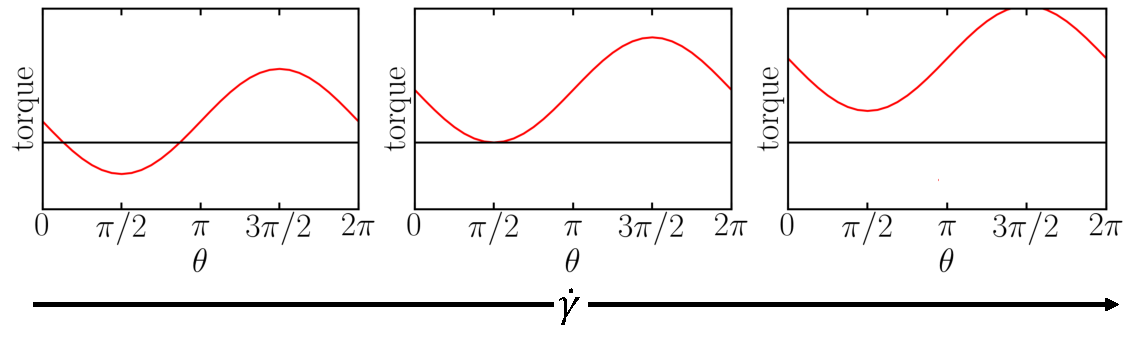
\includegraphics[scale=0.85]{/Users/taiga/Projects/lab/thesis/components/chapter3/figs/sum_torque.pdf}
        \caption{せん断速度の大きさの違いによる粒子にはたらくトルクの分類.
        黒線は$N_z = 0$を表す.
        $\dot{\gamma}_c$はbottom heavy性によるトルクの絶対値の最大値と流体から受けるトルクが等しくなる場合のせん断速度を表す.}
        \label{fig:sum_torque}
    \end{figure}
\noindent
$\dot{\gamma} < \dot{\gamma}_c$の場合には,
bottom heavy性によるトルクが支配的となり,Fig.\ref{fig:sum_torque}(a)のように,
トルクの和が0となる$0 \leq \theta < \pi / 2$の間の角度で粒子の進行方向が固定され,
粒子は回転しないことが予想される.
また,Fig.\ref{fig:sum_torque}(b)のように,
流体から受けるトルクが,bottom heavy性によるトルクの大きさの最大値と等しい値となる場合は,
粒子の進行方向は$\theta = \pi / 2$に固定され,粒子は回転しないことが予想される.
せん断速度がその値よりも大きくなると,Fig.\ref{fig:sum_torque}(c)のように,
流体から受けるトルクが支配的となり,粒子が定常的に回転することが予想される.
このように,流体から受けるトルクとbottom heavy性によるトルクの釣り合いから,粒子の進行方向が異方的になることが予想される.
